% No modificar estas líneas de código, por favor dirigirse a APÉNDICE más abajo.

            \newpage
            \addtocontents{toc}{\setlength{\cftbeforesecskip}{9pt} \protect\renewcommand{\protect\cftsecfont}{\bfseries}}
            \addtocontents{toc}{\cftpagenumbersoff{section}} 
            \phantomsection\addcontentsline{toc}{section}{APÉNDICES}
            \addtocontents{toc}{\cftpagenumberson{section}} 
            
            \newcommand{\apex}[1]
            {
                \newpage
                \vspace*{\fill}
                \section{#1}
                \label{apx:#1}
                \vspace*{\fill}
                \newpage
            }
            
            \appendix
            \renewcommand{\thesection}{\arabic{section}}
            \addtocontents{toc}
            {
                \protect\renewcommand{\protect\cftsecfont}{\normalfont}%
                \protect\renewcommand{\protect\cftsecpresnum}{Apéndice }
                \setlength{\cftsecnumwidth}{2.3cm}
                \setlength{\cftbeforesecskip}{-8pt}%
            }
            
            \setcounter{page}{1}
            \setcounter{figure}{0}
            \setcounter{table}{0}
            \titleformat{\section}{\bfseries\normalsize\flushright}{\MakeUppercase{\textbf{APÉNDICE }\thesection}}{0em}{\\ \MakeUppercase}
            \captionsetup{list=no} % Para que no aparezca en índice general 
            
%------------------------
%
%       APÉNDICE
%
%------------------------
\apex{Entrevista al área de mantenimiento}
\label{apx:1}
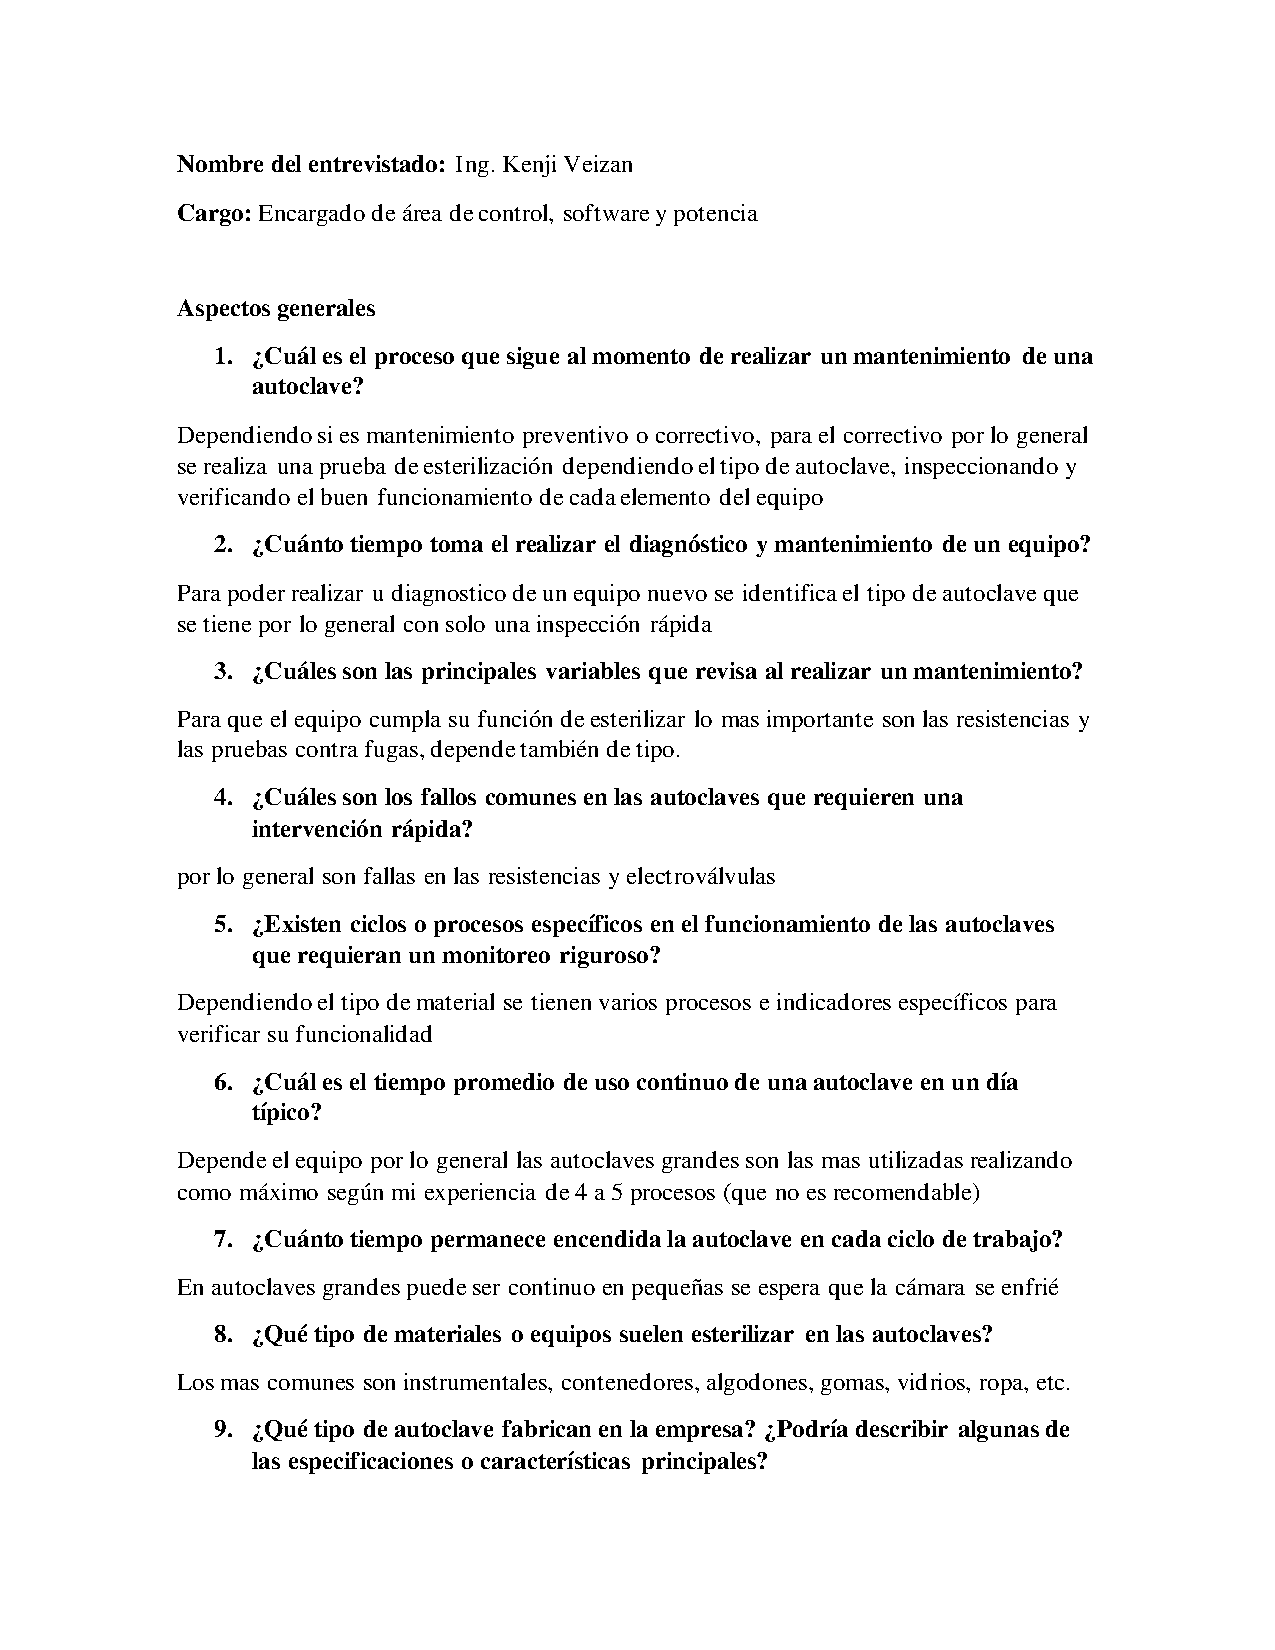
\includepdf[pages={1,2,3}]{PDFs/Entrevista.pdf}
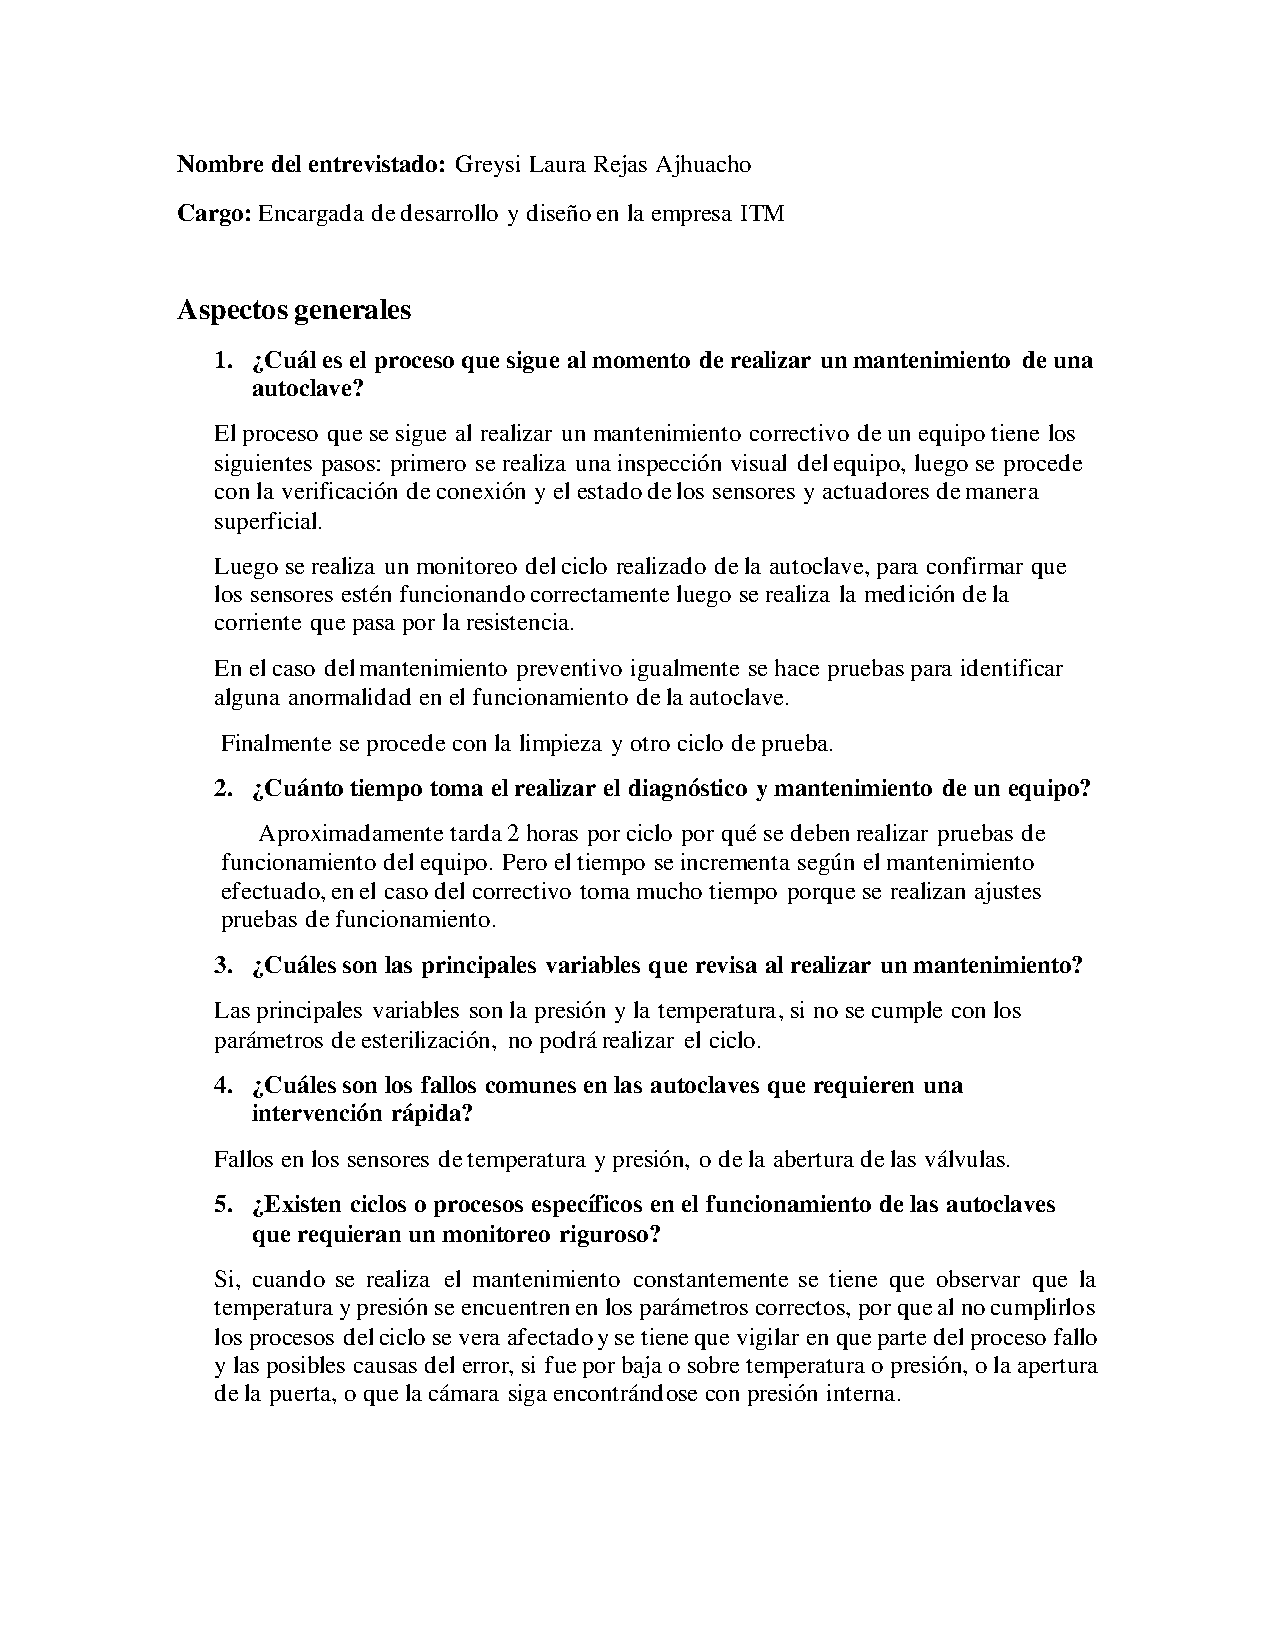
\includepdf[pages={1,2,3}]{PDFs/EntrevistaG.pdf}

\apex{Diagrama del sistema electrónico}
\label{apx:2}
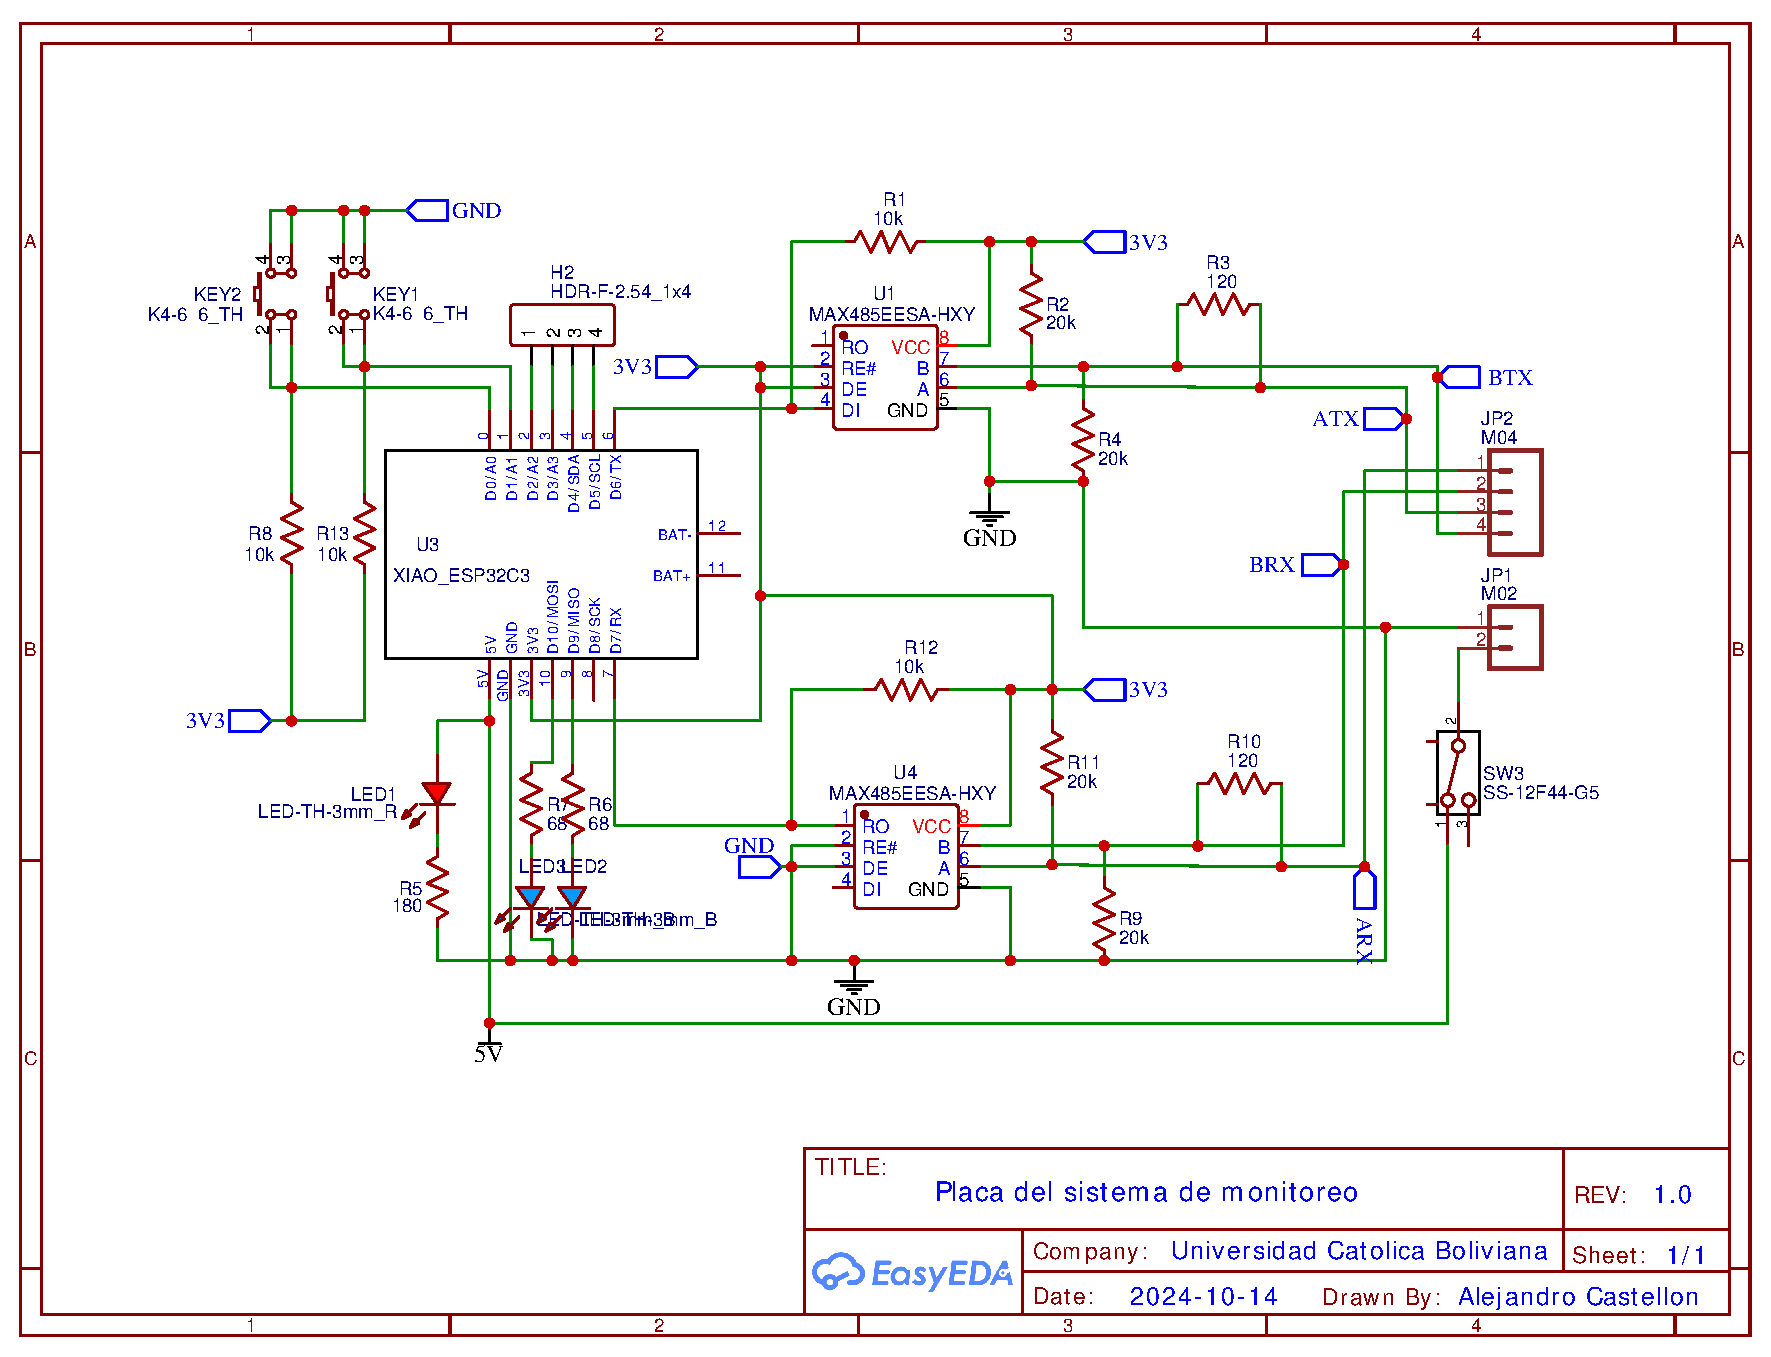
\includepdf[pages={1}]{PDFs/diagram_elec.pdf}

\apex{Diagrama de flujo}
\label{apx:3}
\begin{figure}[hpt]
    \centering
    % Título de figura
    \caption{Diagrama de flujo}
        % imagen 1
        \subfloat[Inicio]{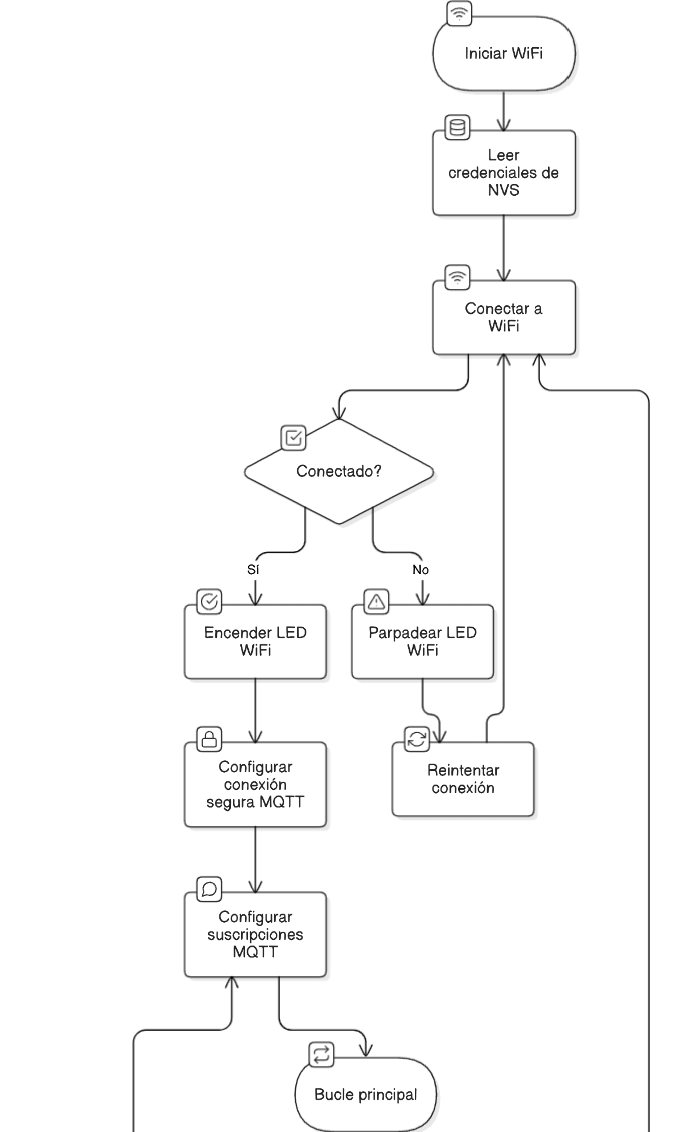
\includegraphics[width=0.4\columnwidth]{Figuras/bloques1.png}}
        % separaciones | agregar una de las opciones entre cada par de imágenes
            \qquad      % figuras en la misma linea
            %\par        % siguiente línea
        % imagen 2
        \subfloat[Bucle]{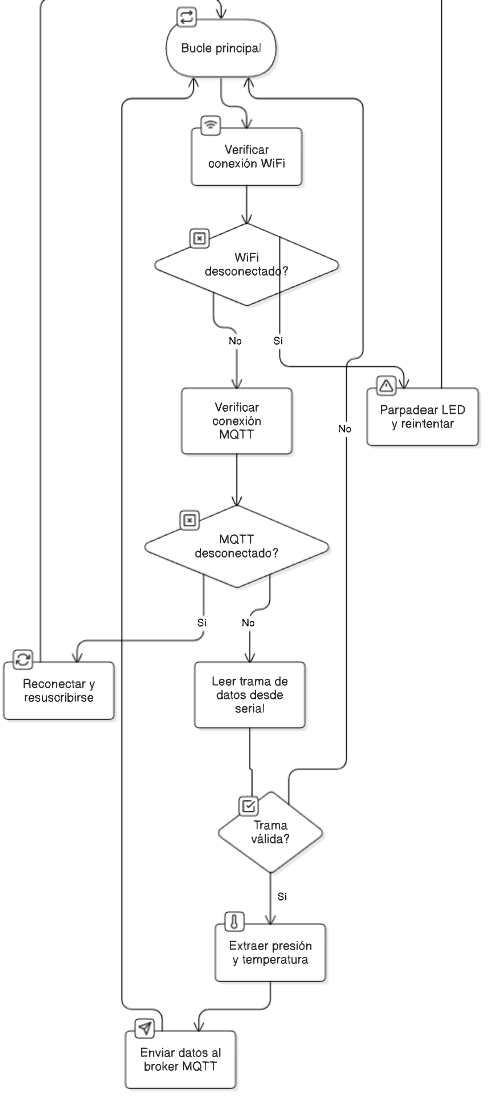
\includegraphics[width=0.4\columnwidth]{Figuras/bloques2.png}}\\
    \centering{\textbf{Fuente:} Elaboración propia (2024)}
    \label{fig:flujo}
\end{figure}

\apex{Planos mecánicos}
\label{apx:4}
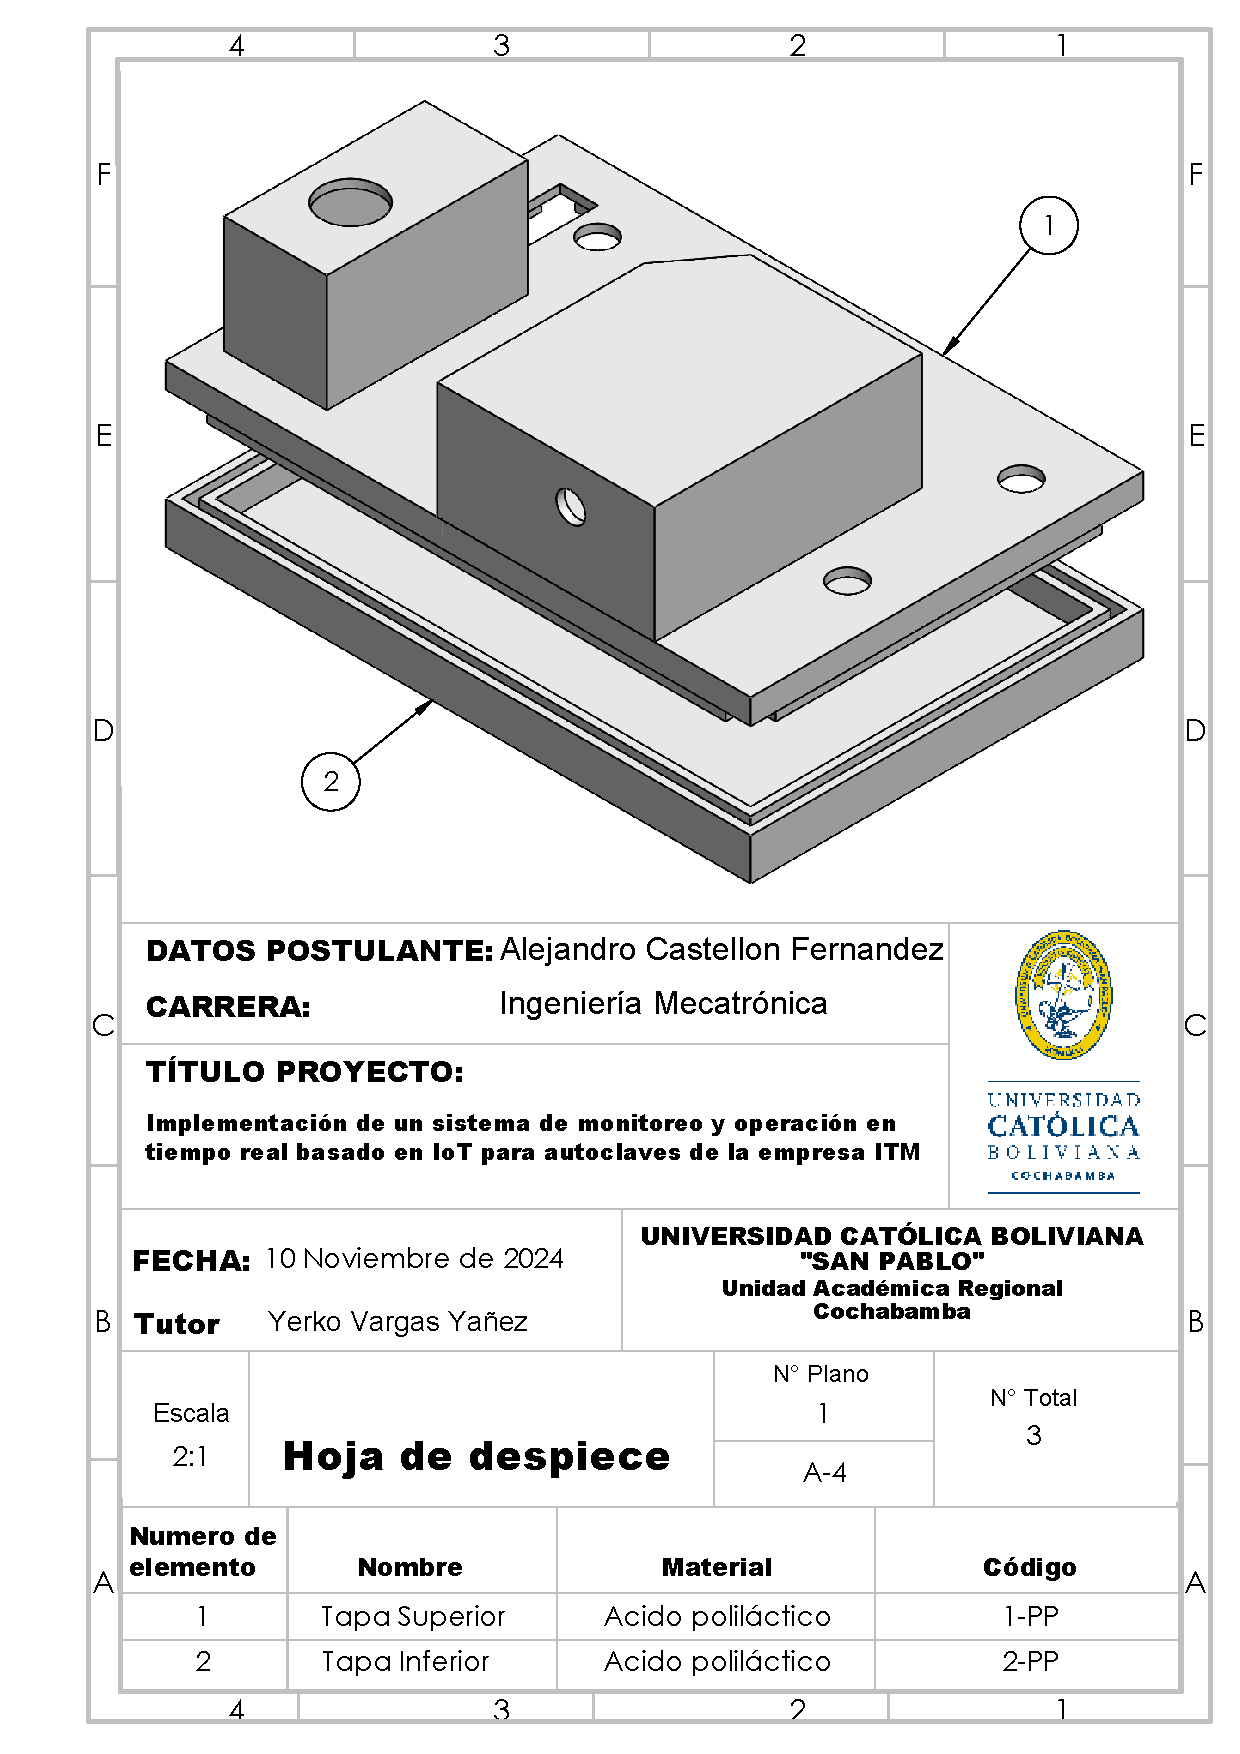
\includepdf[pages={1}]{PDFs/Plano1.PDF}
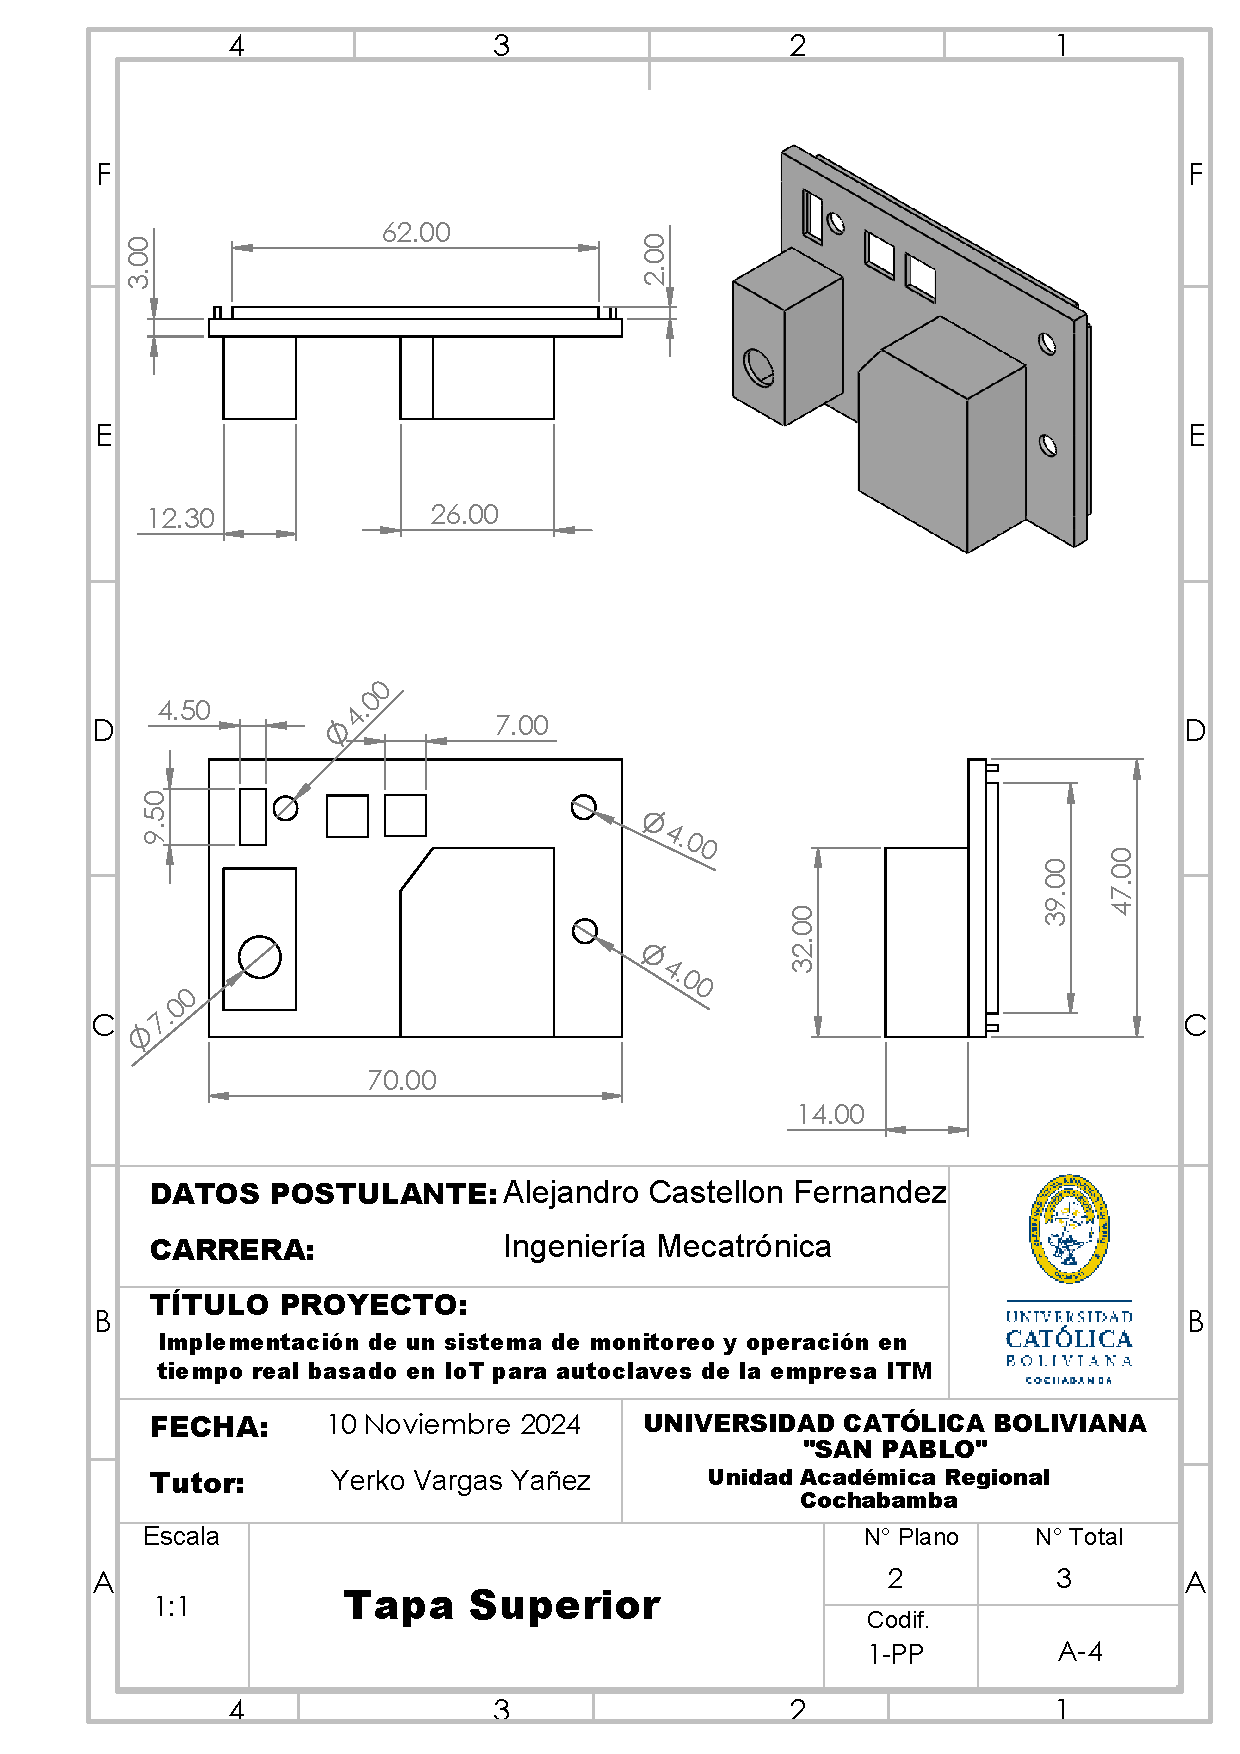
\includepdf[pages={1}]{PDFs/Plano2.PDF}
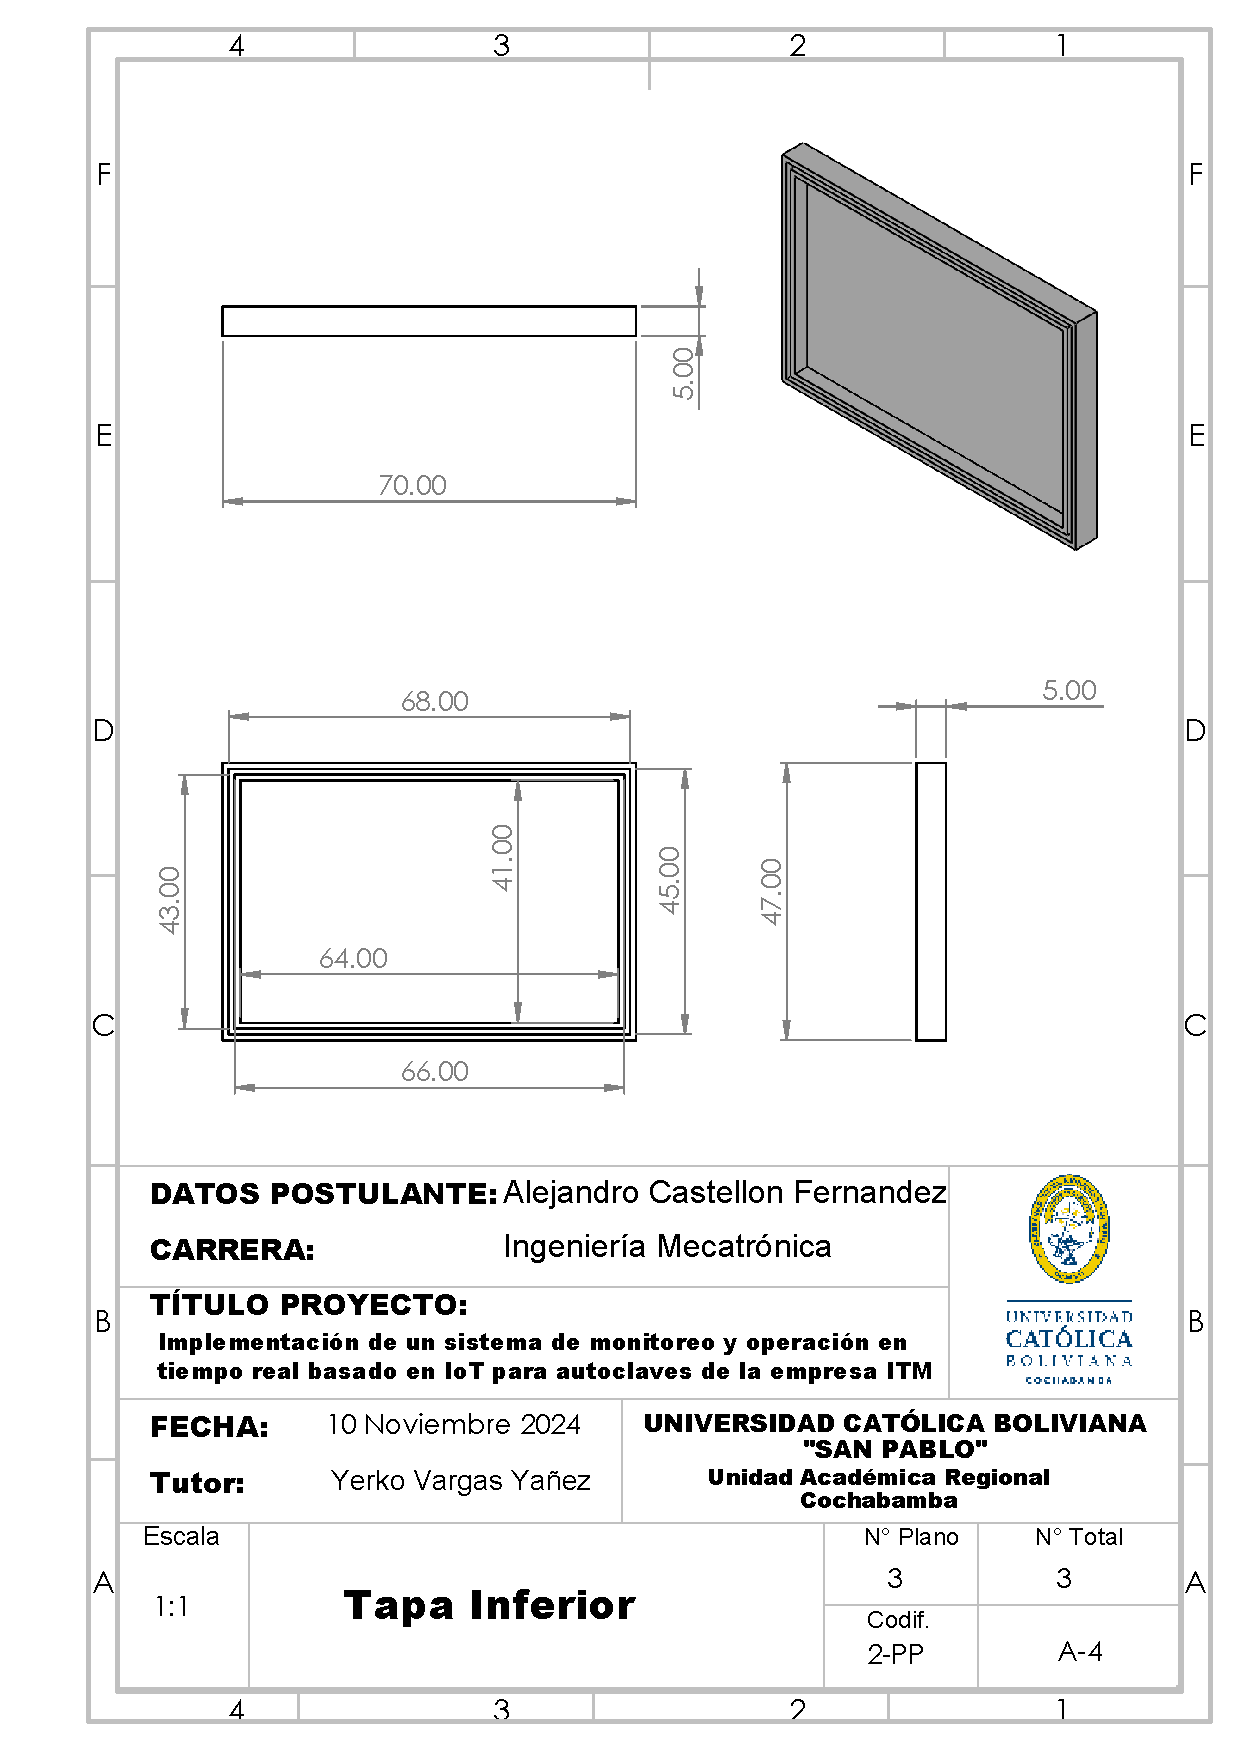
\includepdf[pages={1}]{PDFs/Plano3.PDF}

%Caso usted quisiera adicionar pequeñas líneas de código tal cual fueron introducidas por su persona, puede utilizar el formato a continuación.

%\begin{lstlisting}[frame=single]
  % suma de los elementos de un vector
 % z = 0;
 % n = length(v);
  %for i=1:1:n
  %  z = z + v[i];
 % end
%\end{lstlisting}

